\section{Scelte progettuali}
Di seguito verranno illustrate le principali scelte progettuali effettuate durante la realizzazione del progetto.

\subsection{Server}

\subsubsection{Architettura}
L'architettura del server è stata scelta tra due soluzioni, che sono state trattate più in dettaglio durante il Laboratorio di Reti di Calcolatori:

\begin{enumerate}
	\item multithread sincrona con I/O bloccante (\texttt{Sockets} di \texttt{Java IO});
	\item monothread sincrona con I/O non bloccante (\texttt{Selectors} di \texttt{Java NIO}).
\end{enumerate}

Le due soluzioni hanno pregi e difetti complementari, ma il trade-off principale è tra \textbf{velocità} e \textbf{scalabilità}. Ai fini di questo progetto didattico è stata ritenuta più importante la reattività, garantita (sotto carichi non eccessivi) dalla prima soluzione.
\medskip \\
Possiamo dividere il server in due livelli: \textbf{interfaccia} e \textbf{core}.

\begin{enumerate}
	\item A livello di interfaccia si trovano:
		\begin{enumerate}
			\item Il socket TCP del server
			\item L'API del servizio di registrazione utente
			\item Il servizio RMI di notifiche push.
		\end{enumerate}
	\item A livello core si trovano:
		\begin{enumerate}
			\item Il thread pool di client handlers
			\item I manager di utenti, documenti e indirizzi IP multicast.
		\end{enumerate}
\end{enumerate}

Per ogni client che si connette, il server riserva un thread, che si occuperà di gestire la connessione TCP per l'intero tempo di vita del client.

L'\textbf{automa a stati} del client di \texttt{TURING} è stato implementato con tre stati interni ad ogni client handler, perché non si può fare affidamento sulla buona scrittura del client.
\medskip \\
L'invio di messaggi \textbf{multicast} viene effettuato tramite un \texttt{datagramChannel} che viene aperto quando c'è almeno un utente che sta modificando il documento, e chiuso quando nessuno lo sta più modificando.

\newpage

\begin{center}
	\begin{figure}[ht!]
		\makebox[\textwidth]{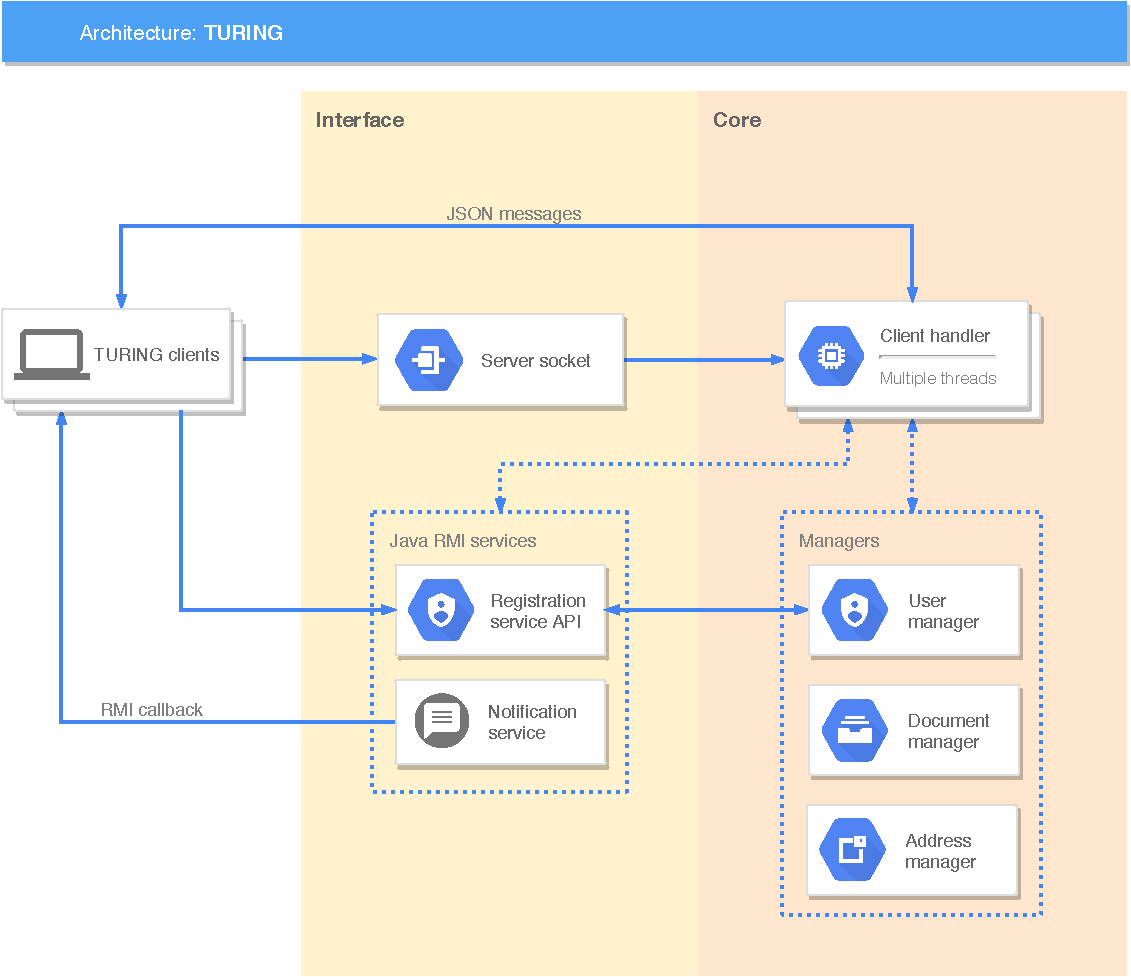
\includegraphics[width=0.75\paperwidth]{img/turing_architecture.pdf}}
		\caption{Architettura di \texttt{TURING} e interazioni tra le varie componenti.}
	\end{figure}
\end{center}

\subsubsection{Strutture dati}
Le principali strutture dati utilizzate sono tabelle hash (per gli utenti e per i documenti) e alberi (per gli indirizzi). Verranno approfondite nella sezione di gestione della concorrenza.

\subsubsection{Protocollo di terminazione}
\sloppy
Quando il server viene terminato (a parte il caso eccezionale del segnale \texttt{SIGKILL}), viene avviata in un nuovo thread una routine di cleanup, dove:
\begin{itemize}
	\item viene chiuso il socket del server;
	\item viene attesa la terminazione dei thread del pool per un tempo massimo pari al doppio del tempo di risveglio dei socket verso i client; se dopo questo tempo qualche thread è ancora in esecuzione, viene terminato forzatamente;
	\item vengono cancellati tutti i file di testo salvati dagli utenti, in quanto il server non mantiene uno stato da caricare al riavvio.
\end{itemize}

\subsubsection{Organizzazione dei documenti}
I documenti vengono salvati come file di testo codificati nello standard \texttt{UTF-8}, rispettando la seguente gerarchia (utente $\rightarrow$ documento $\rightarrow$ sezione):

\medskip

\dirtree{%
	.1 data/.
	.2 Michele/.
	.3 relazione\_turing/.
	.4 1.
	.4 2.
	.4 3.
	.2 Dante Alighieri/.
	.3 Divina Commedia/.
	.4 1.
	.4 2.
	.4 \dots.
	.4 100.
	.3 De vulgari eloquentia/.
	.4 1.
	.4 2.
}


\subsection{Client}

\subsubsection{Architettura}
L'architettura del client è più semplice: effettua richieste in formato JSON e resta in attesa di una risposta. Il thread grafico è aggiornato all'occorrenza dal metodo \texttt{invokeLater}. Durante la normale esecuzione, il client è single threaded; viene generato al bisogno un thread per la ricezione di messaggi multicast, durante la modifica di un documento.

\medskip

L'interfaccia grafica si adatta automaticamente alle dimensioni dello scher\-mo, ed è stato cercato di renderla il più coerente e intuitiva possibile.

\medskip

Dalla schemata di registrazione e login si può accedere all'area personale di \texttt{TURING}, dove ogni utente può creare nuovi documenti, invitare altri utenti alla modifica, e in una tabella dinamica vede i documenti che può modificare, con la lista delle sezioni e informazioni aggiuntive, come il nome del creatore del documento (indispensabile nel caso di documenti omonimi) e un'icona che indica se il documento è stato condiviso o no. La tabella si aggiorna in tempo reale quando si viene invitati alla modifica di un nuovo documento (con apposito messaggio di notifica), ma è anche possibile forzare un aggiornamento manuale tramite il tasto ``refresh".

\medskip

Dopo che una sezione di un documento è stata selezionata per la modifica, viene visualizzata la schermata di lavoro, nella quale è possibile modificare il testo precedentemente salvato, chattare con gli utenti che stanno modificando lo stesso documento, salvare le modifiche o ignorarle.

\begin{center}
	\begin{figure}[ht!]
		\makebox[\textwidth]{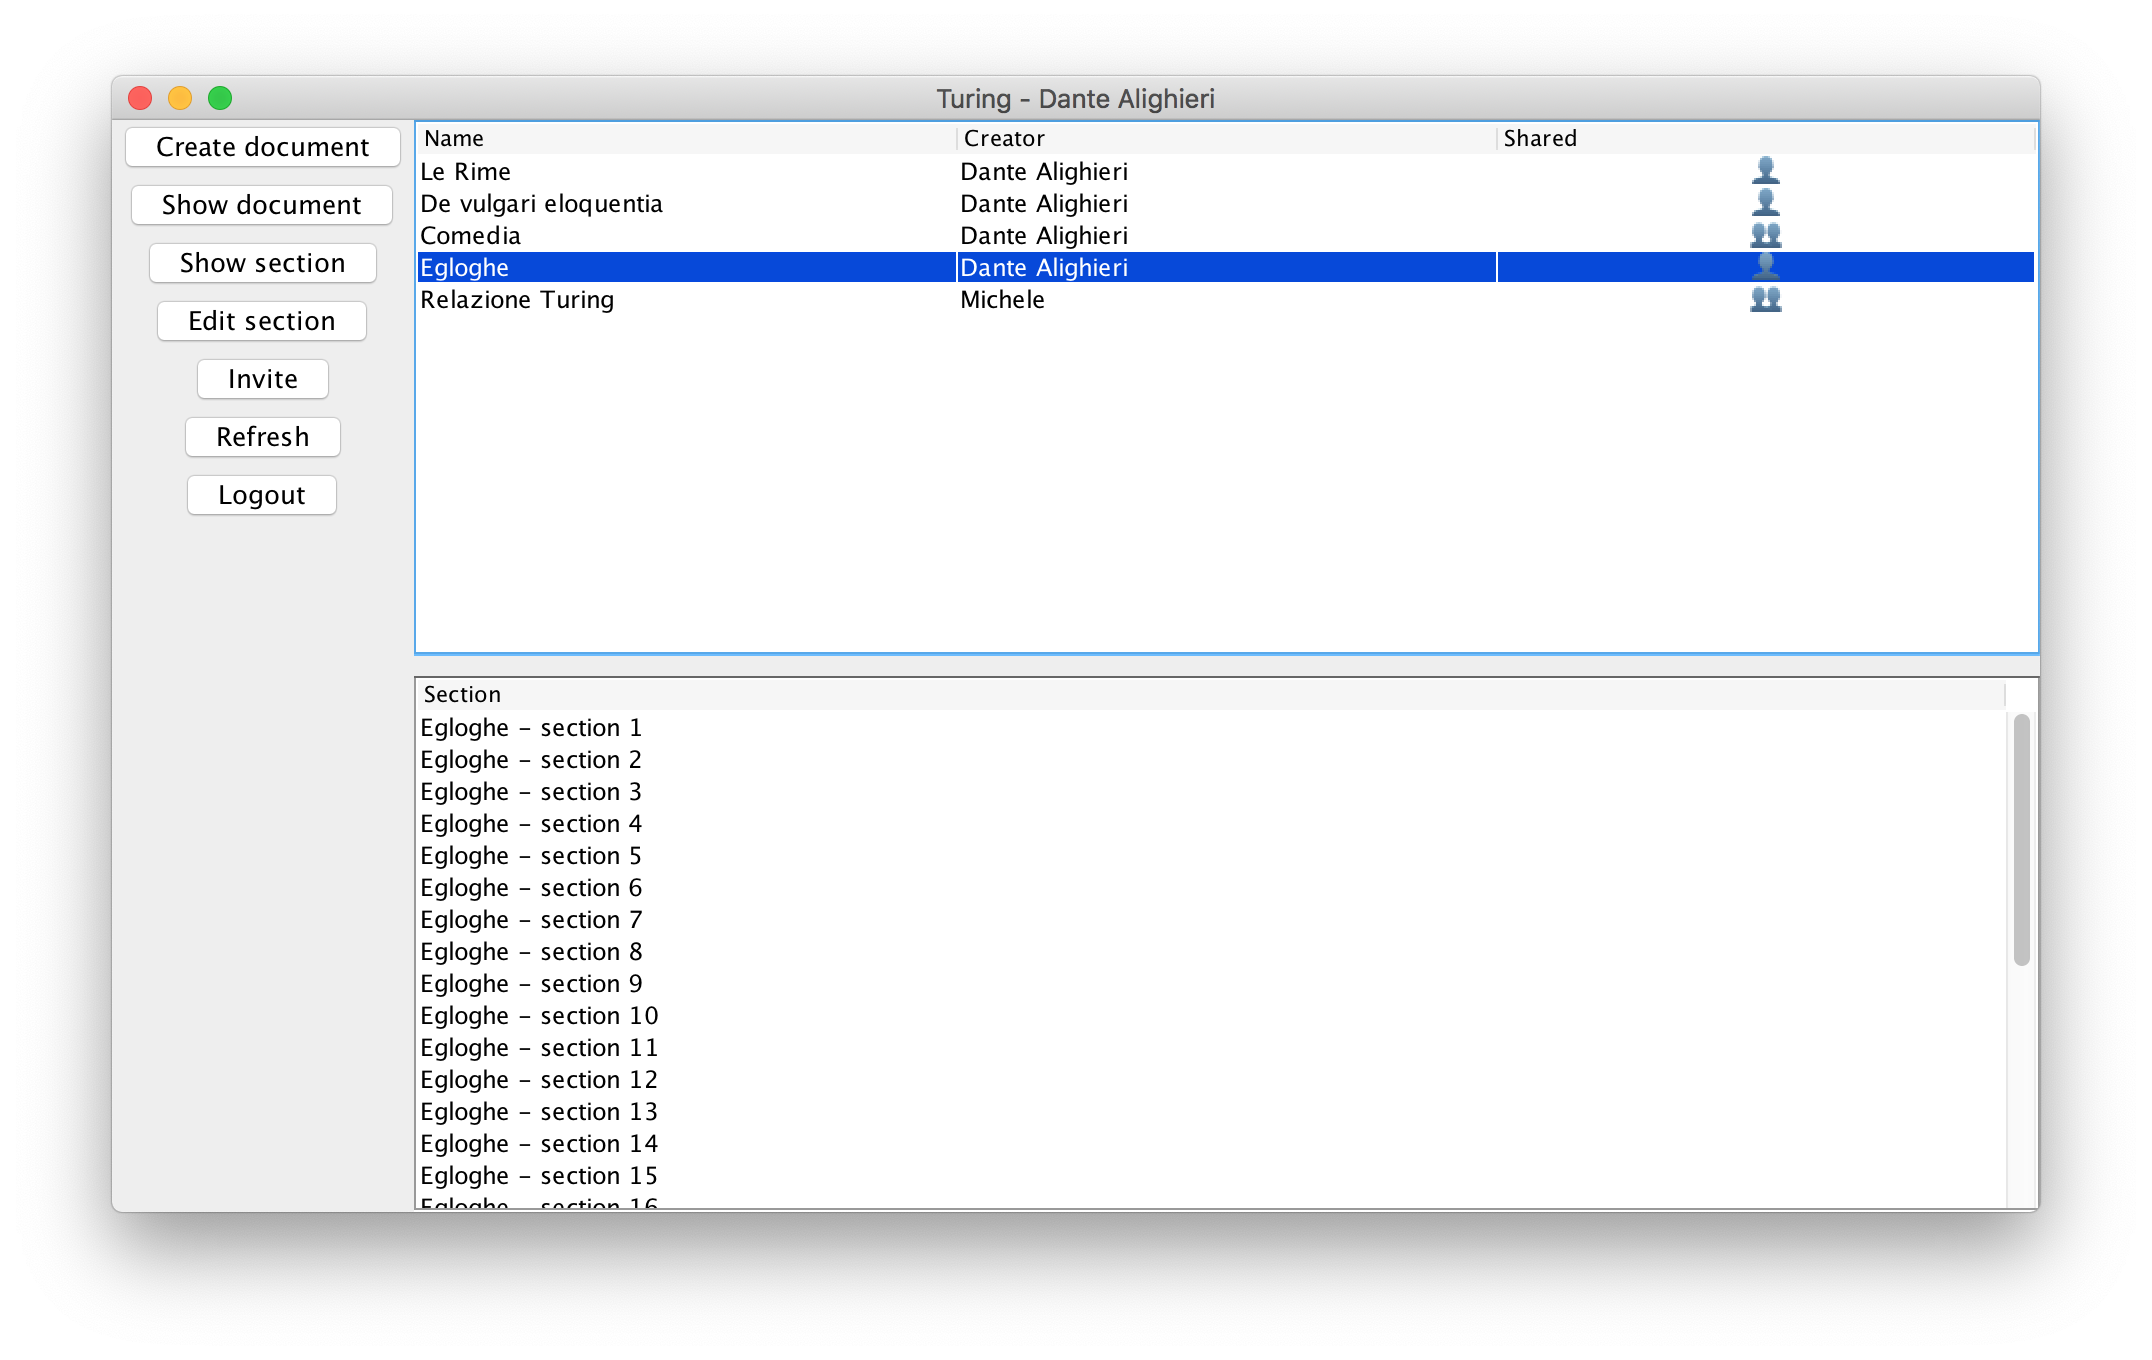
\includegraphics[width=1.4\linewidth]{screenshots/documents.png}}
		\caption{Elenco dei documenti di Dante Alighieri. Notare le icone per indicare la condivisione o meno di un documento.}
	\end{figure}

	\begin{figure}[ht!]
		\makebox[\textwidth]{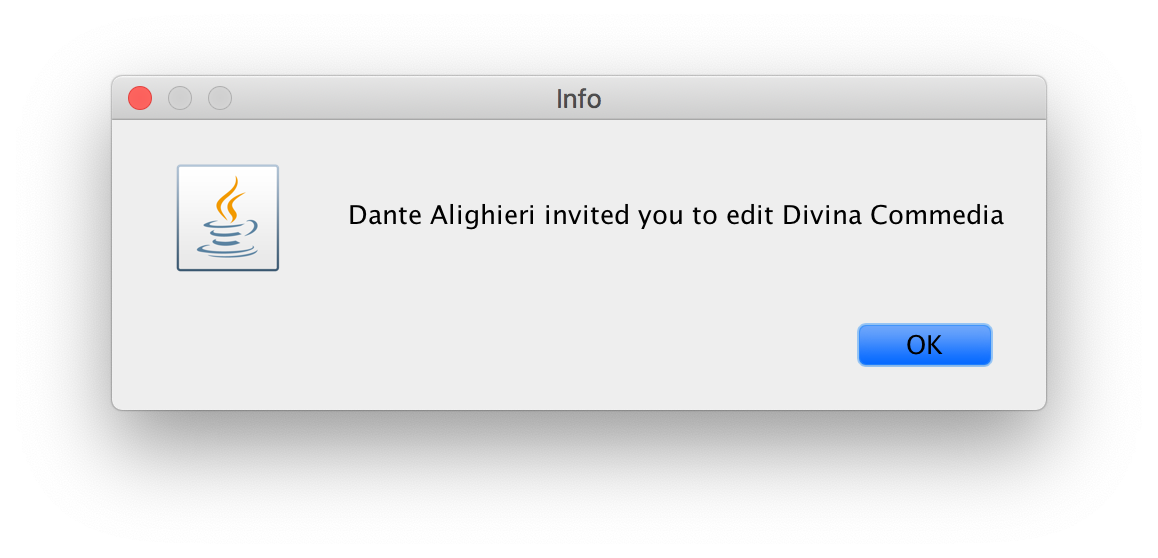
\includegraphics[width=0.70\linewidth]{screenshots/notification.png}}
		\caption{Notifica che indica che Michele è stato invitato alla modifica della Divina Commedia da parte di Dante Alighieri.}
	\end{figure}

	\begin{figure}[ht!]
		\makebox[\textwidth]{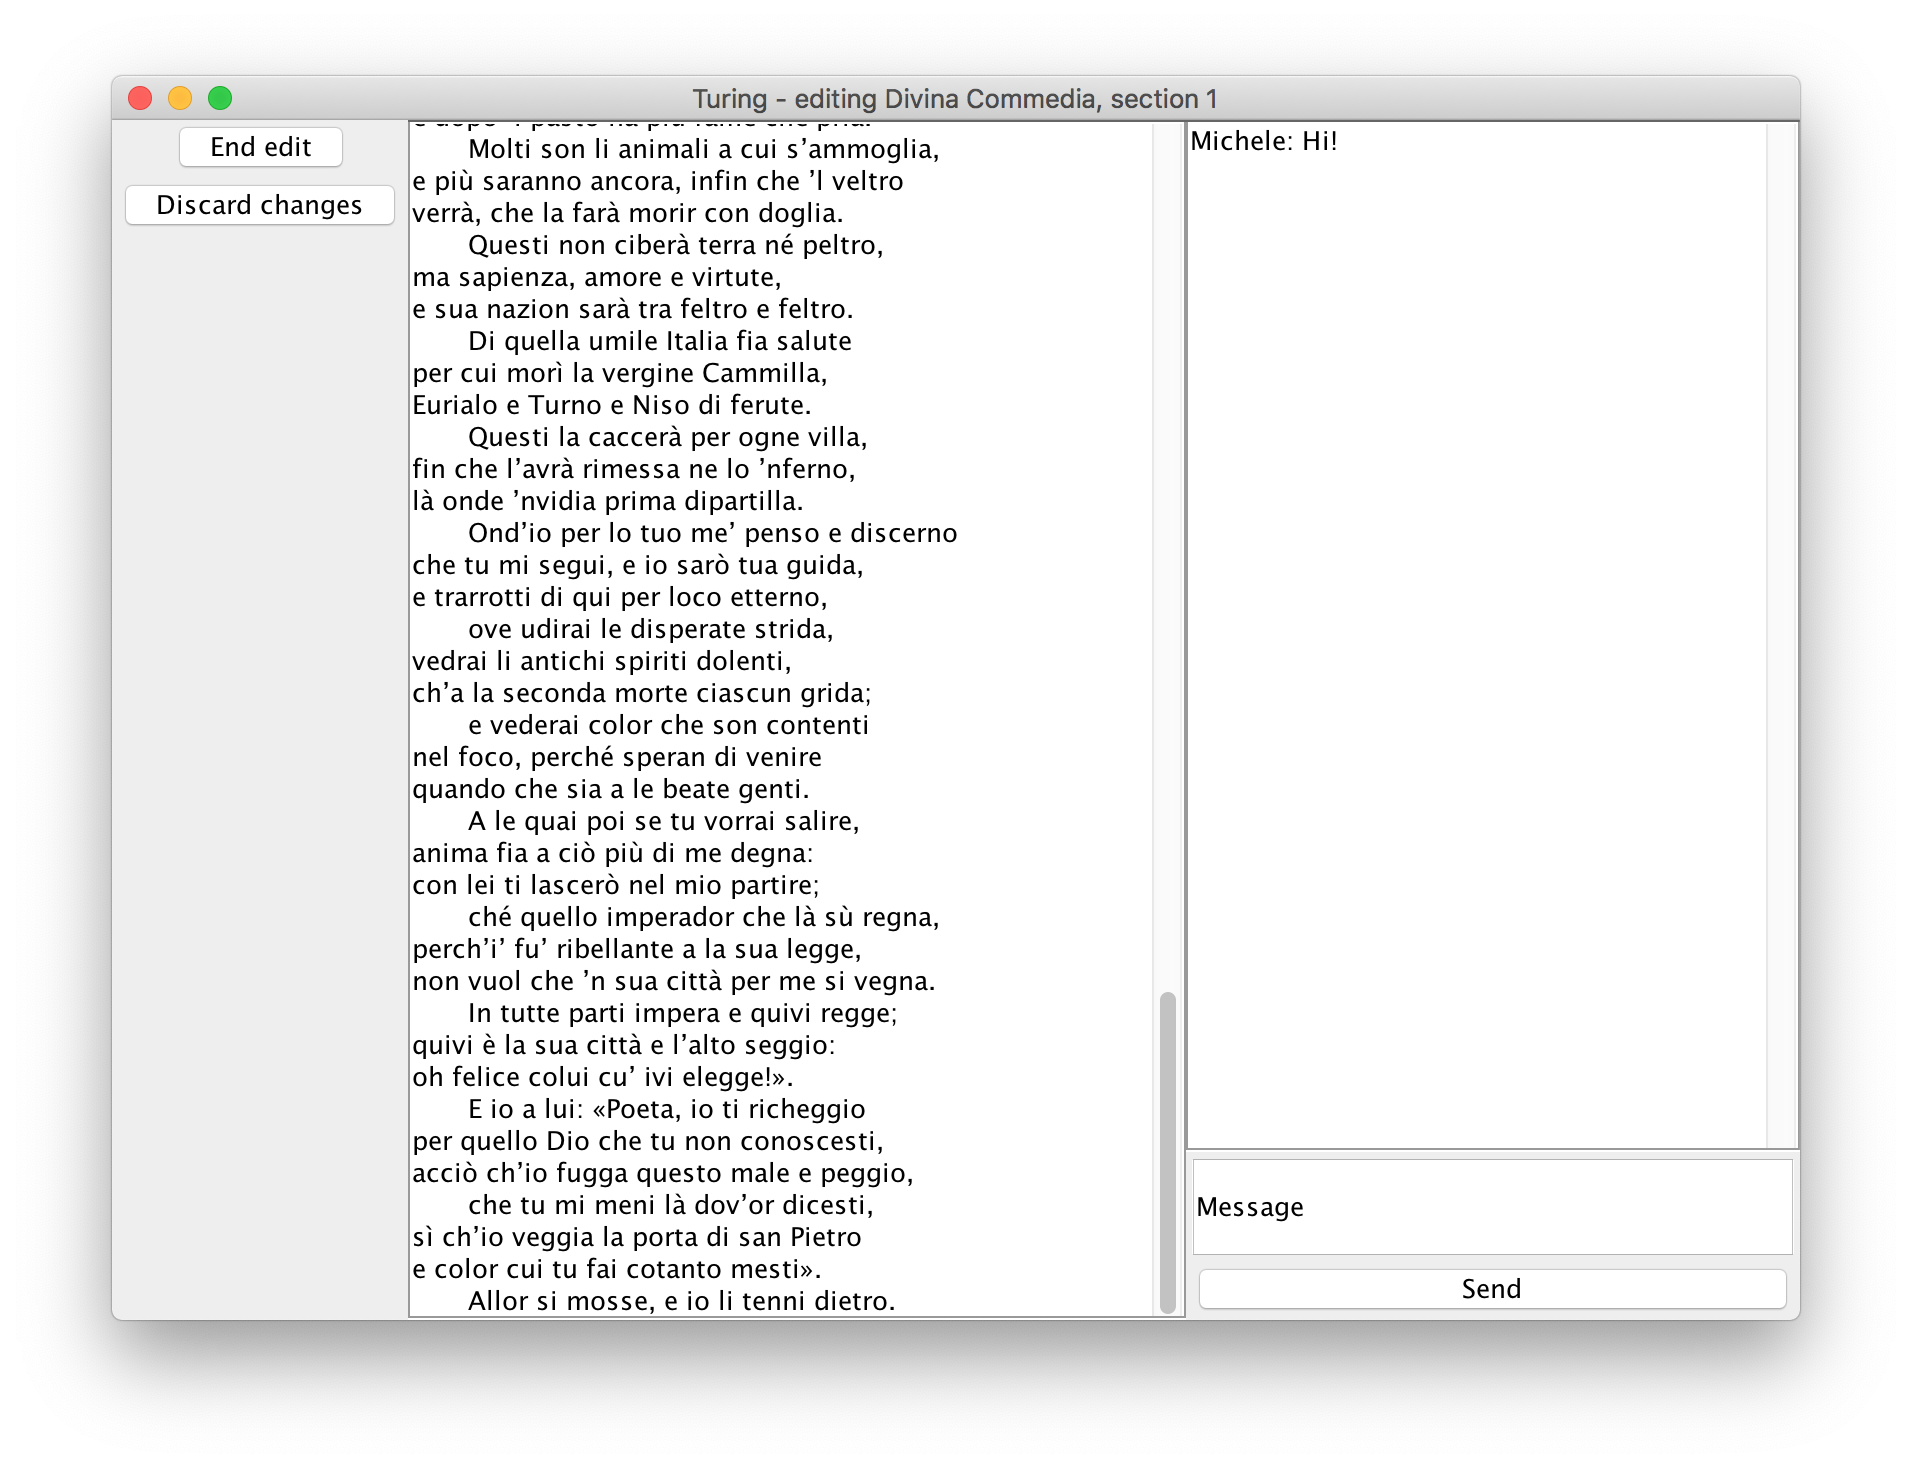
\includegraphics[width=1.20\linewidth]{screenshots/workspace.png}}
		\caption{Dante Alighieri modifica la prima sezione della Divina Commedia, mentre gli arriva un messaggio in chat da Michele.}
	\end{figure}
\end{center}

\newpage


\subsection{Comunicazione client-server}
Per la comunicazione client-server è stata adottata una tecnica a scambio di messaggi sincrona. I messaggi sono in formato JSON, e vengono inviati attraverso una connessione TCP. La scelta del formato JSON al posto degli oggetti Java serializzati permette una \textbf{maggiore interoperabilità}, consentendo in un futuro momento di scrivere client per \texttt{TURING} in qualsiasi linguaggio di programmazione\footnote{A patto di modificare la parte di registrazione utente, che è stata richiesta esplicitamente in Java RMI.}.

\medskip

Il formato dei messaggi è indicato nel file \texttt{message\_format.txt} all'interno della cartella \texttt{format}, assieme ad un esempio di messaggio che richiede al server la creazione di un documento.

\subsection{Librerie}
Sia nel client che nel server è stata utilizzata una libreria per la creazione e il parsing di oggetti JSON, scaricabile dalla repository di Maven (\href{https://mvnrepository.com/artifact/org.json/json}{\textbf{link}}).
